\documentclass[a5paper]{article}
\usepackage[a5paper, top=8mm, bottom=8mm, left=8mm, right=8mm]{geometry}

\usepackage{polyglossia}
\setdefaultlanguage[babelshorthands=true]{russian}

\usepackage{fontspec}
\setmainfont{FreeSerif}
\newfontfamily{\russianfonttt}[Scale=0.7]{DejaVuSansMono}

\usepackage[font=scriptsize]{caption}

\usepackage{amsmath}
\usepackage{amssymb,amsfonts,textcomp}
\usepackage{color}
\usepackage{array}
\usepackage{hhline}
\usepackage{cite}
\usepackage{textcomp}

\usepackage[hang,multiple]{footmisc}
\renewcommand{\footnotelayout}{\raggedright}

\PassOptionsToPackage{hyphens}{url}\usepackage[xetex,linktocpage=true,plainpages=false,pdfpagelabels=false]{hyperref}
\hypersetup{colorlinks=true, linkcolor=blue, citecolor=blue, filecolor=blue, urlcolor=blue, pdftitle=1, pdfauthor=, pdfsubject=, pdfkeywords=}

\newlength\Colsep
\setlength\Colsep{10pt}

\usepackage{tabu}

\usepackage{graphicx}
\usepackage{indentfirst}
\usepackage{multirow}
\usepackage{subfig}
\usepackage{footnote}
\usepackage{minted}

\newcommand{\todo}[1] {
\begin{center}\textcolor{red}{TODO: #1}\end{center}
}

\newcommand{\attribution}[1] {
	\vspace{-5mm}\begin{flushright}\begin{scriptsize}%\textcolor{gray}
	{\textcopyright\, #1}\end{scriptsize}\end{flushright}
}

\sloppy
\pagestyle{plain}

\title{Лекция 5:  Моделирование поведения}
\author{Юрий Литвинов\\\small{yurii.litvinov@gmail.com}}
\date{}

\begin{document}

\maketitle
\thispagestyle{empty}

\section{Введение}

В этой лекции мы закончим обсуждение UML, рассмотрев диаграммы, которые используются на этапе разработки, или более конкретно, для моделирования поведения. Речь пойдёт не только про UML, но и некоторые другие формализмы, используемые для этой цели.

\section{Диаграммы конечных автоматов}

Диаграммы конечных автоматов (также известные как диаграммы состояний) --- эт на самом деле несколько упрощённые диаграммы Харела, предложенные им ещё в 1987 году, коорые попали в UML с минимальными изменениями. Это второй вид диаграмм UML, имеющий исполнимую семантику. Предназначены эти диаграммы для моделирования поведения <<реактивных>> систем (или частей системы), то есть систем, которые находятся в некоторых чётко определённых состояниях, от которых зависит их поведение, и могут реагировать на события, переходя из состояния в состояние и, возможно, делая при переходах полезную работу. Примеры реактивных систем --- это сетевое соединение (которое может быть открыто, закрыто, открываемо в данный момент, закрываемо, и в зависимости от этого передаёт или не передаёт пакеты), либо классический пример с торговым автоматом, с которого начинался рассказ про моделирование вообще.

Выглядят диаграммы конечных автоматов так:

\begin{center}
	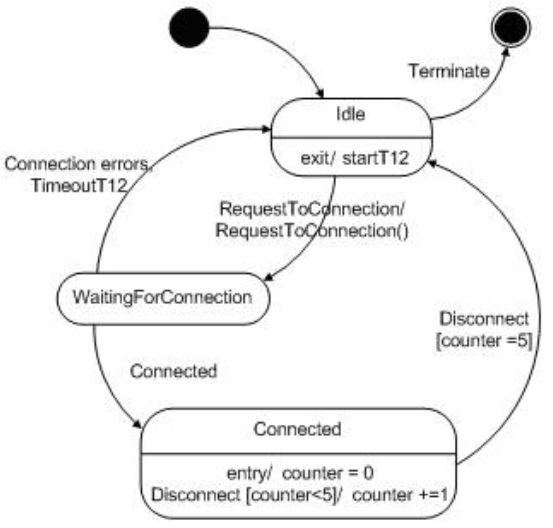
\includegraphics[width=0.5\textwidth]{stateTransitionExample.png}
\end{center}

Прямоугольниками со скруглёнными углами рисуются состояния, у состояния есть имя и (опционально) действия, выполняемые в состоянии (например, действие по выходу или внутренний переход по событию, как у Connected --- получив событие Disconnect, оно проверяет счётчик, и если счётчик меньше 5, он увеличивается на 1 и мы остаёмся в том же состоянии). Состояния связаны переходами, над переходом пишется событие, которое инициирует переход и, опционально, стражник (guard) (логическое условие, которое должно быть истинно, чтобы переход состоялся) и действие, выполняемое при переходе. События со стражниками должны быт взаимно исключающими, недетерминированные автоматы считаются некорректными. Есть псевдосостояния начала и конца, переход из псевдосостояния начала происходит мгновенно, переход в состояние конца заканчиввает исполнение.

Внешне диаграммы конечных автоматов похожи на диаграммы активностей, но есть важные семантические различия:

\begin{itemize}
	\item На диаграмме активностей рисуются активности, система в них не задерживается, а сразу переходит дальше; на диаграмме конечных автоматов рисуются состояния --- стабильные отрезки жизненного цикла объекта, в которых он находится большую часть времени и может из них выйти только если что-то произойдёт;
	\item Полезная работа на диаграммах активностей производится в активностях, на диаграммах автоматов --- как правило, при переходе;
	\item Диаграммы активностей моделируют один метод объекта (или какую-то функцию или что-то такое), диаграммы конечных автоматов --- целый объект (состояния моделируются полями объекта).
\end{itemize}

Более подробно про синтаксис:

\begin{center}
	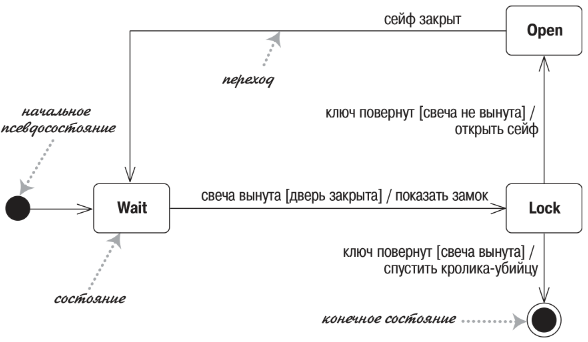
\includegraphics[width=\textwidth]{stateTransitionSyntax.png}
	\attribution{М. Фаулер, UML. Основы}
\end{center}

Внутри состояния могут быть:

\begin{itemize}
	\item entry activity --- то, что делается при входе в состояния по любому из переходов;
	\item exit activity --- то, что делается при выходе из состояния по любому исходящему переходу (и входная, и выходная деятельность --- это, как правило, вызовы метода);
	\item do activity --- деятельность, выполняющаяся всегда, когда система находится в таком-то состоянии (например, попытки подключения к сети для мобильного телефона);
	\item внутренний переход --- переход по событию, который ведёт в то же состояние и не приводит к срабатыванию entry и exit activity. Переход вполне может быть полноценным переходом в то же состояние (рисуется как петля в графе), тогда entry и exit activity работают как обычно, хоть состояние и не меняется.
\end{itemize}

Событие, кстати, это нечто внешнее по отношению к системе, на что система может реагировать. Примеры событий --- действие пользователя, сетевой пакет, считывание символа (если речь идёт об автоматном лексическом анализаторе, который, кстати, хоть и несколько необычный, но тоже пример реактивной системы, которая прекрасно моделируется конечными автоматами).

Надпись на переходе имеет следующий синтаксис: \verb|[<trigger> [‘,’ <trigger>]* [‘[‘ <guard>’]’] [‘/’ <behavior-expression>]]| --- один переход может реагировать на несколько событий сразу, иметь опционального стражника (в квадратных скобках) и через слеш действие (вызов метода или отсылку к диаграмме активностей, которая поясняет, что нужно делать при переходе).

Вот более содержательный пример автомата из работ Д.В. Кознова. Пример демонстрирует порядок работы мобильного телефона, начиная с включения и ввода PIN-кода и заканчивая подключением к сети:

\begin{center}
	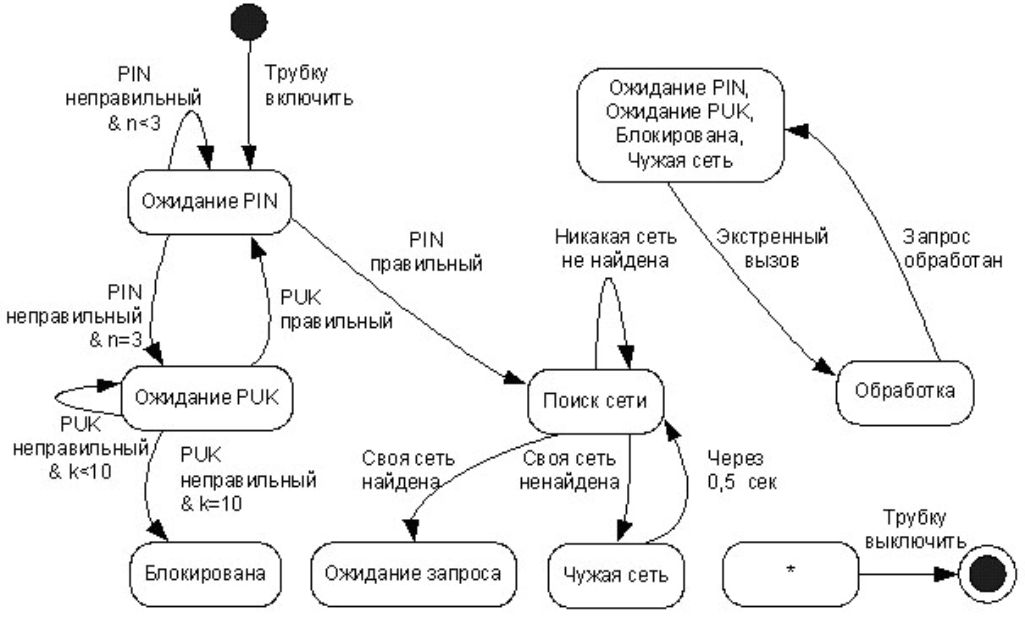
\includegraphics[width=0.7\textwidth]{stateTransitionExample2.png}
\end{center}

Тут используется неканоничный синтаксис с псевдосостоянием ``все состояния'', из которого ведёт переход в конечное псевдосостояние (чтобы не рисовать переход из каждого состояния в конечное) и используются не совсем каноничные надписи над переходами. Связано это с тем, что в те времена, когда на матмехе делались работы по диаграммам конечных автоматов, UML 2 ещё не было, а в UML первых версий синтаксис диаграмм конечных автоматов был менее проработан.

Более продвинутый синтаксис современных диаграмм конечных автоматов позволяет нарисовать пример выше более канонично. Есть вложенные состояния с переходами сразу из всех внутренних состояний:

\begin{center}
	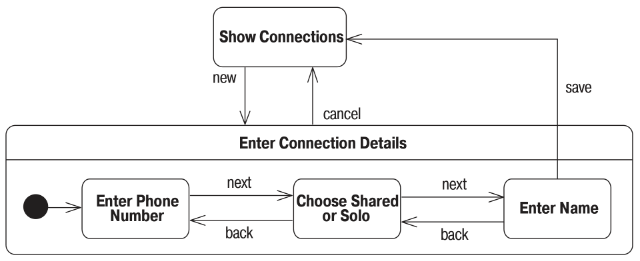
\includegraphics[width=\textwidth]{stateTransitionNestedStates.png}
	\attribution{М. Фаулер, UML. Основы}
\end{center}

Тут состояние <<Enter connection details>> содержит внутри свой конечный автомат, который начинает работать со стартового псевдосостояния когда выполняется переход <<new>>. При этом переход <<save>> возможен только из состояния <<Enter Name>>, а вот переход <<cancel>> возможен из любого вложенного состояния (это замена нестандартному псевдосостоянию со звёздочкой из диаграммы выше).

Ещё бывают параллельные состояния и псевдосостояние истории:

\begin{center}
	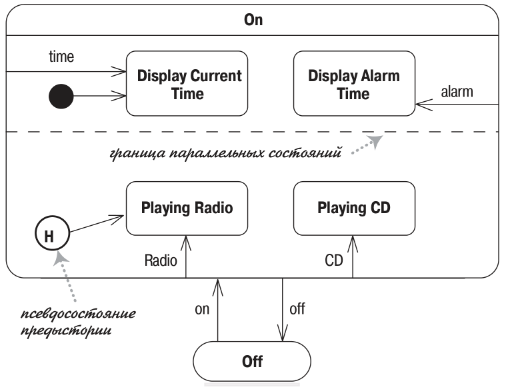
\includegraphics[width=0.7\textwidth]{stateTransitionParallelStates.png}
	\attribution{М. Фаулер, UML. Основы}
\end{center}

Это часы с радио и будильником. Проигрывание звука и время работают независимо, поэтому по сути это два автомата, работающих параллельно (что и показывает горизонтальная прерывистая линия, разделяющая параллельные подавтоматы). Стрелки от объемлющего состояния к вложенным означают, что система, находясь в объемлющем состоянии, реагирует на такие-то события и изменяет внутреннее состояние (например, часы по умолчанию показывают текущее время, но если пользователь нажал на кнопку <<будильник>>, начинает показывать время, на которое будильник установлен). Псевдосостояние истории запоминает последнее вложенное состояние, в котором находился автомат, и возвращает автомат в него. Например, часы по умолчанию включают радио, но если пользователь включил воспроизведение компакт-дисков (если кто помнит, что это такое) и выключил часы, то при следующем включении они снова будут проигрывать компакт-диски.

А вот так рисуются активности внутри состояния:

\begin{center}
	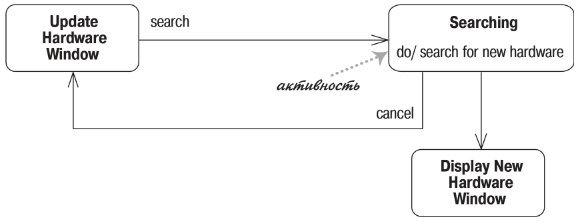
\includegraphics[width=\textwidth]{stateTransitionInternalEventExample.png}
	\attribution{М. Фаулер, UML. Основы}
\end{center}

А вот так --- внутренние переходы и entry/exit-события, о которых шла речь выше:

\begin{center}
	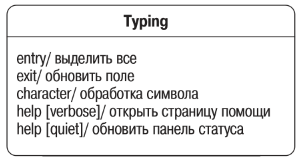
\includegraphics[width=0.5\textwidth]{stateTransitionInternalEvents.png}
	\attribution{М. Фаулер, UML. Основы}
\end{center}

Как видим, синтаксис очень похож на то, что пишется при переходе.

\subsection{Генерация кода}

Конечные автоматы хороши тем, что по ним можно легко и приятно генерировать код, в силу их стандартизованной семантики. Рассмотрим наш пример с кроликом-убийцей:

\begin{center}
	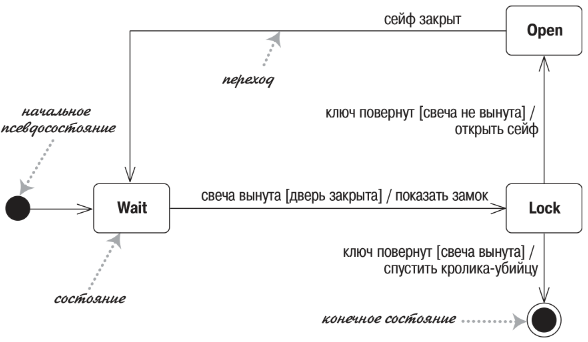
\includegraphics[width=\textwidth]{stateTransitionSyntax.png}
	\attribution{М. Фаулер, UML. Основы}
\end{center}

Первый, самый простой способ сгенерировать код --- это сгенерировать гигантский switch, внутри которого чуть менее гигантские switch-и. Внешний switch --- по текущему состоянию автомата, внутренние --- по событиям, на которые находясь в данном состоянии автомат может реагировать. Внутри --- проверка условий стражников, выполнение действия по переходу и переход в следующее состояние. Состояние моделируется enum-ом, хранящимся как поле объекта. Для нашего примера получится что-то такое:

\begin{minted}{java}
public void handleEvent(PanelEvent anEvent) {
    switch (currentState) {
        case PanelState.Open:
            switch (anEvent) {
                case PanelEvent.SafeClosed:
                    currentState = PanelState.Wait;
            }
            break;
        case PanelState.Wait:
            switch (anEvent) {
                case PanelEvent.CandleRemoved:
                    if (isDoorOpen) {
                        revealLock();
                        currentState = PanelState.Lock;
                    }
            }
            break;
        case PanelState.Lock:
            switch (anEvent) {
                case PanelEvent.KeyTurned:
                    if (isCandleIn) {
                        openSafe();
                        currentState = PanelState.Open;
                    } else {
                        releaseKillerRabbit();
                        currentState = PanelState.Final;
                    }
            }
            break;
    }
}
\end{minted}

Это работает, но если этот код надо сопровождать, никто от него не будет в восторге. Для сколько-нибудь содержательных автоматов получается один метод на тысячи строк. Поэтому можно использовать таблицу состояний и универсальный интерпретатор, который просто ищет в таблице текущее состояние и событие, и выполняет то, что там написано. Вариантов таблиц состояний может быть много, но вот пример из книжки Фаулера:

\begin{center}
	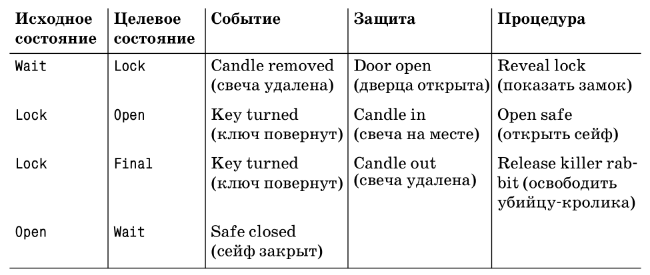
\includegraphics[width=0.5\textwidth]{stateTransitionStateTable.png}
	\attribution{М. Фаулер, UML. Основы}
\end{center}

Таблица состояний обычно либо хранится как файл данных рядом с программой, либо вкомпилируется в исходный код. 

Такой подход очень популярен в лексическом и синтаксическом анализе, но отлаживать или просто понимать такие программы очень тяжело. Поэтому есть ещё один, более объектно-ориентированный способ симулировать автомат: паттерн проектирования <<Состояние>>:

\begin{center}
	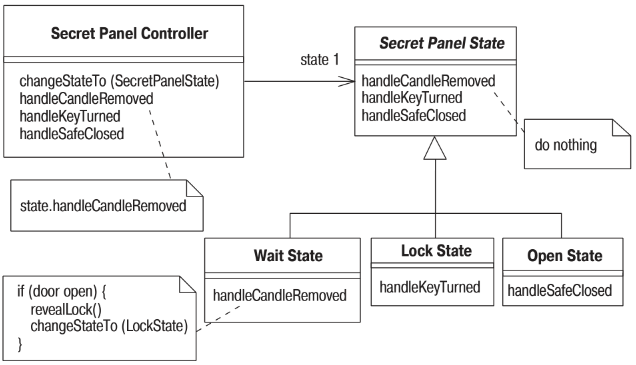
\includegraphics[width=0.5\textwidth]{stateTransitionStatePattern.png}
	\attribution{М. Фаулер, UML. Основы}
\end{center}

Автомат представляется в виде класса, который имеет в качестве поля ссылку на интерфейс <<текущее состояние>>. Этот интерфейс имеет столько методов, сколько всего разных событий может обрабатывать автомат. Интерфейс реализуют конкретные классы, отвечающие за конкретные состояния, они определяют те методы интерфейса, на которые могут реагировать, там уже проверяют условия стражников и выполняют действие при переходе. Каждый такой метод возвращает объект-состояние, в которое должен перейти автомат дальше. То есть, по сути, это тот же switch, где самый большой switch (по состояниям) спрятан в таблицу виртуальных методов. Такой подход делает реализацию автомата более-менее читаемой, ограничивает ответственность каждого класса только одним состоянием и позволяет очень легко добавить новые состояния, поэтому очень популярен при <<ручной>> реализации автоматов.

\section{Диаграммы последовательностей}

Следующий тип диаграмм UML, использующийся при моделировании поведения --- это диаграммы последовательностей (sequence diagrams). Они применяются для визуализации взаимодействия между объектами --- передачи сообщений, возврата значений, времени жизни объекта. Выглядят диаграммы следующим образом:

\begin{center}
	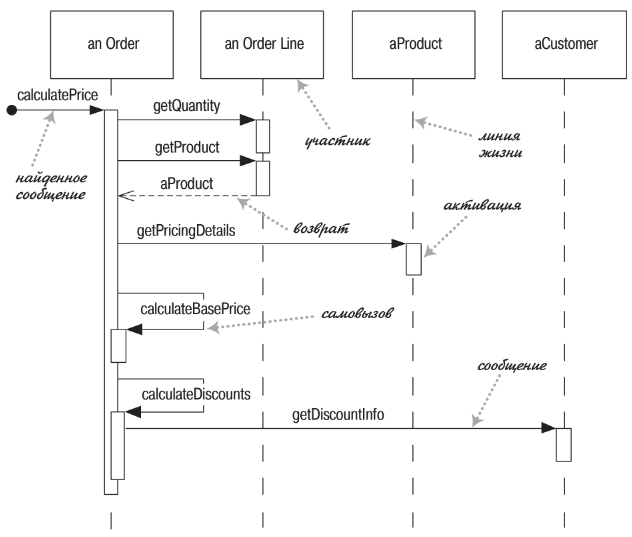
\includegraphics[width=0.9\textwidth]{sequenceDiagramSyntax.png}
	\attribution{М. Фаулер, UML. Основы}
\end{center}

На диаграмме рисуются объекты (обратите внимание, не классы), из каждого объекта выходит \textit{линия жизни} (пунктирная линия), на которой расположены \textit{линии активации} (длинный белый прямоугольник). Линия жизни показывает, когда объект вообще существует в памяти, линия активации --- когда объект занят какой-то работой (то есть работает либо его метод, либо метод, вызванный из его метода, или, более формально, какой-либо из методов объекта находится на стеке вызовов). Линий активации одновременно может быть несколько --- рекурсивные вызовы. Стрелки между линиями активации обозначают сообщения --- как правило, это вызовы методов, и поэтому они ведут в начало соответствующих вызванному методу линий активации. Обратите внимание, что стрелка не может выходить из неактивного объекта и не может входить <<в никуда>>.

Такая диаграмма позволяет разобраться в даже довольно сложных протоколах взаимодействия, поэтому применяется при многопоточном и асинхронном программировании, чтобы визуализировать общение между потоками/асинхронные вызовы. Также такие диаграммы очень популярны при описании телекоммуникационных протоколов (на самом деле, есть отдельный язык MSC (Message Sequence Charts), который применяется независимо от UML, но диаграммы последовательностей являются его почти копией).

Имеется и ряд менее очевидных применений: 

\begin{itemize}
	\item на этапе анализа предметной области для визуализации последовательности коммуникаций между участниками взаимодействия;
	\item на этапе проектирования для составления плана тестирования --- кто в каком порядке кого должен дёргать и кто когда чем должен отвечать;
	\item на этапе отладки, для визуализации логов работающей системы.
\end{itemize}

Ещё немного синтаксических подробностей:

\begin{center}
	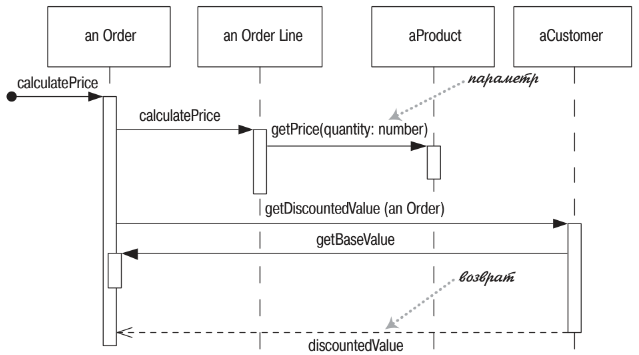
\includegraphics[width=0.6\textwidth]{sequenceDiagramSyntax2.png}
	\attribution{М. Фаулер, UML. Основы}
\end{center}

На этом примере видна передача параметров в сообщении (обратите внимание, что параметрами могут быть сами участники взаимодействия, например, <<an Order>> передаётся в <<aCustomer>>, тот самый <<an Order>>, из линии активации которого выходит сообщение). Здесь же показан возврат значения из вызова, <<discountedValue>>.

\subsection{Примеры}

Пример диаграммы последовательностей из реального проекта:

\begin{center}
	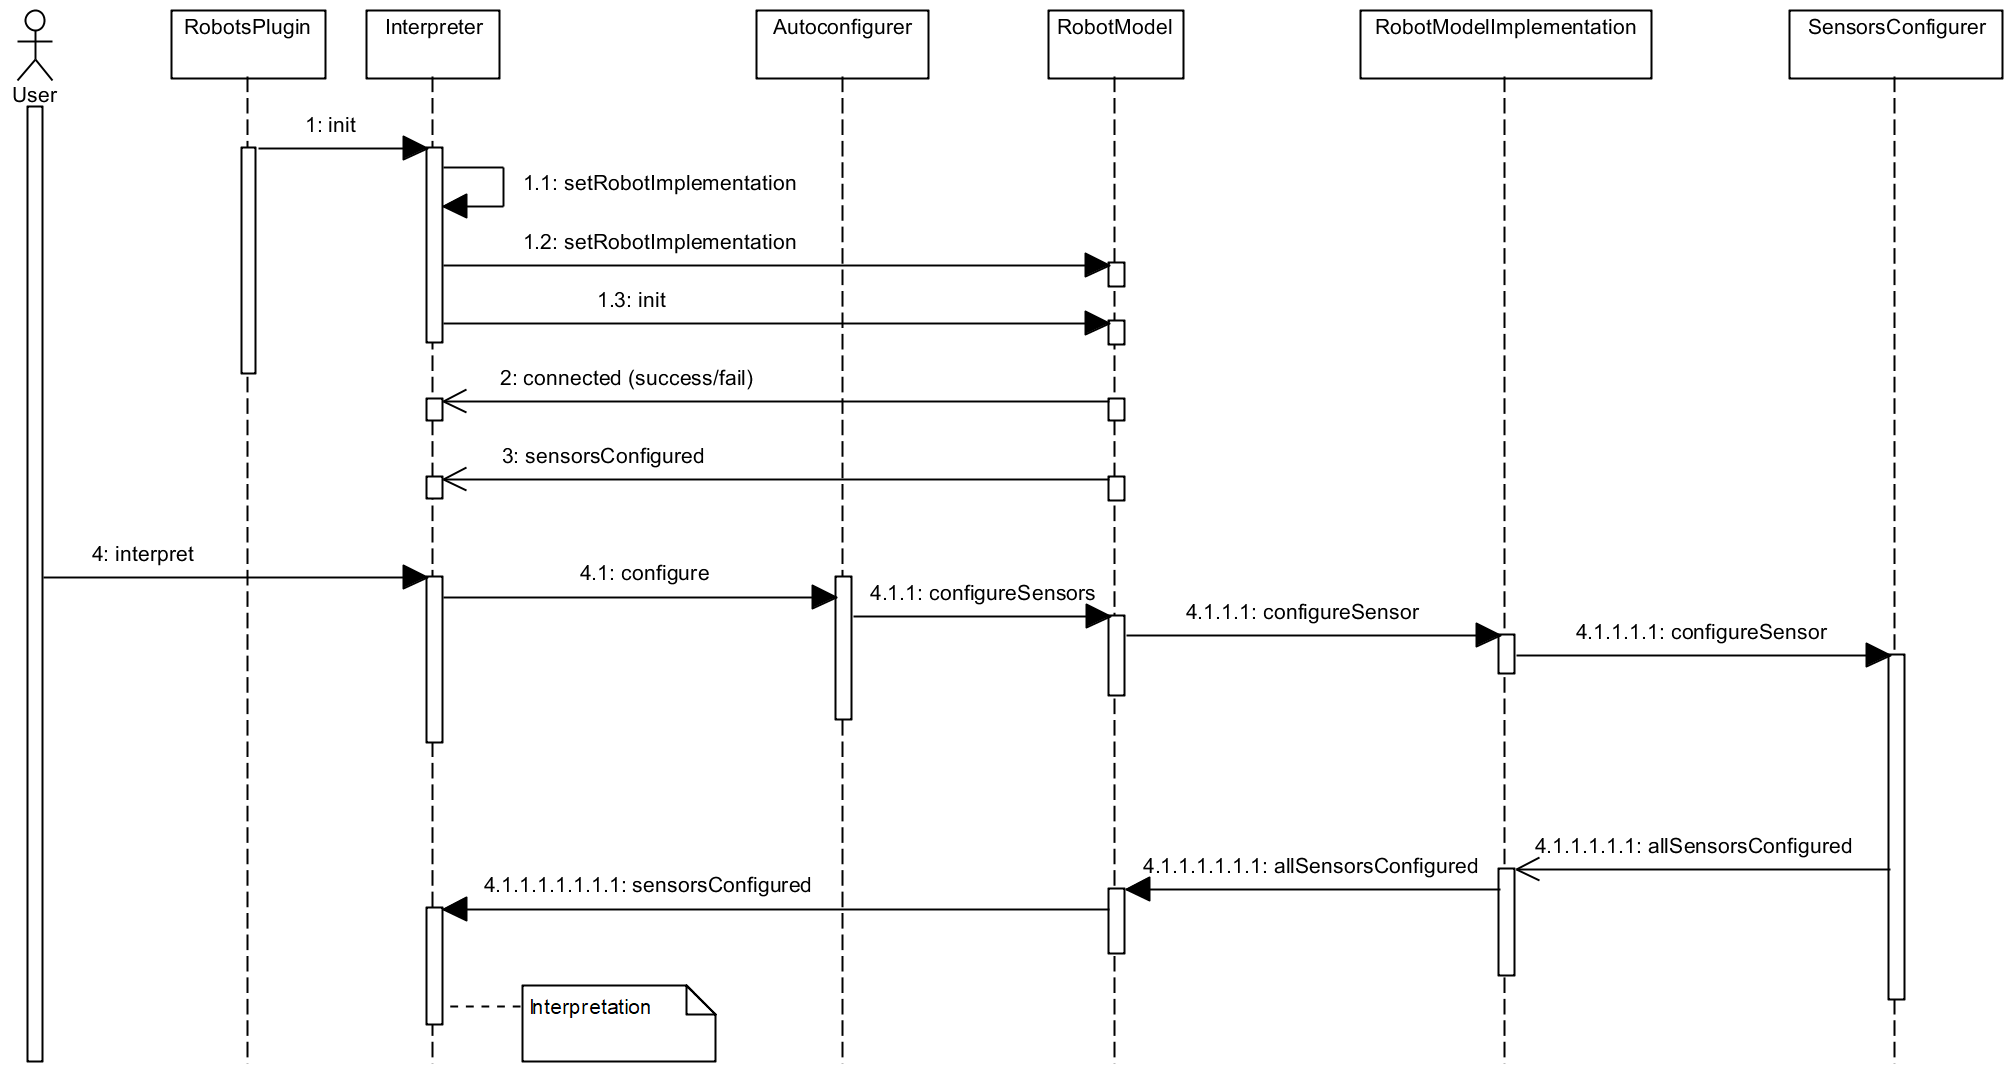
\includegraphics[width=\textwidth]{sequenceDiagramExample.png}
\end{center}

Показывается сценарий конфигурирования робота при запуске интерпретации программы в среде программирования роботов. Сначала система инициализируется, выбирает реализацию подсистемы связи с роботом (исходя из того, с каким роботом сейчас работает пользователь), посылает ему команду инициализации, после чего асинхронно получает два сигнала --- подключение удалось/не удалось (<<connected>>) и сенсоры сконфигурированы на роботе в конфигурации по умолчанию (<<sensorsConfigured>>). Далее становится доступна кнопка <<Interpret>>, пользователь нажимает её и запускает процесс конфигурации сенсоров --- среда программирования смотрит на программу, понимает, какие сенсоры и как там используются, смотрит на настройки и рассчитывает итоговую конфигурацию сенсоров, которые и шлёт на робот. Дальше она дожидается асинхронного ответа о том, что все сенсоры готовы к работе, и начинает собственно интерпретацию программы. Как видим, протокол инициализации довольно сложен, но на диаграмме он вполне обозрим, и это очень помогает при отладке.

Ещё один пример:

\begin{center}
	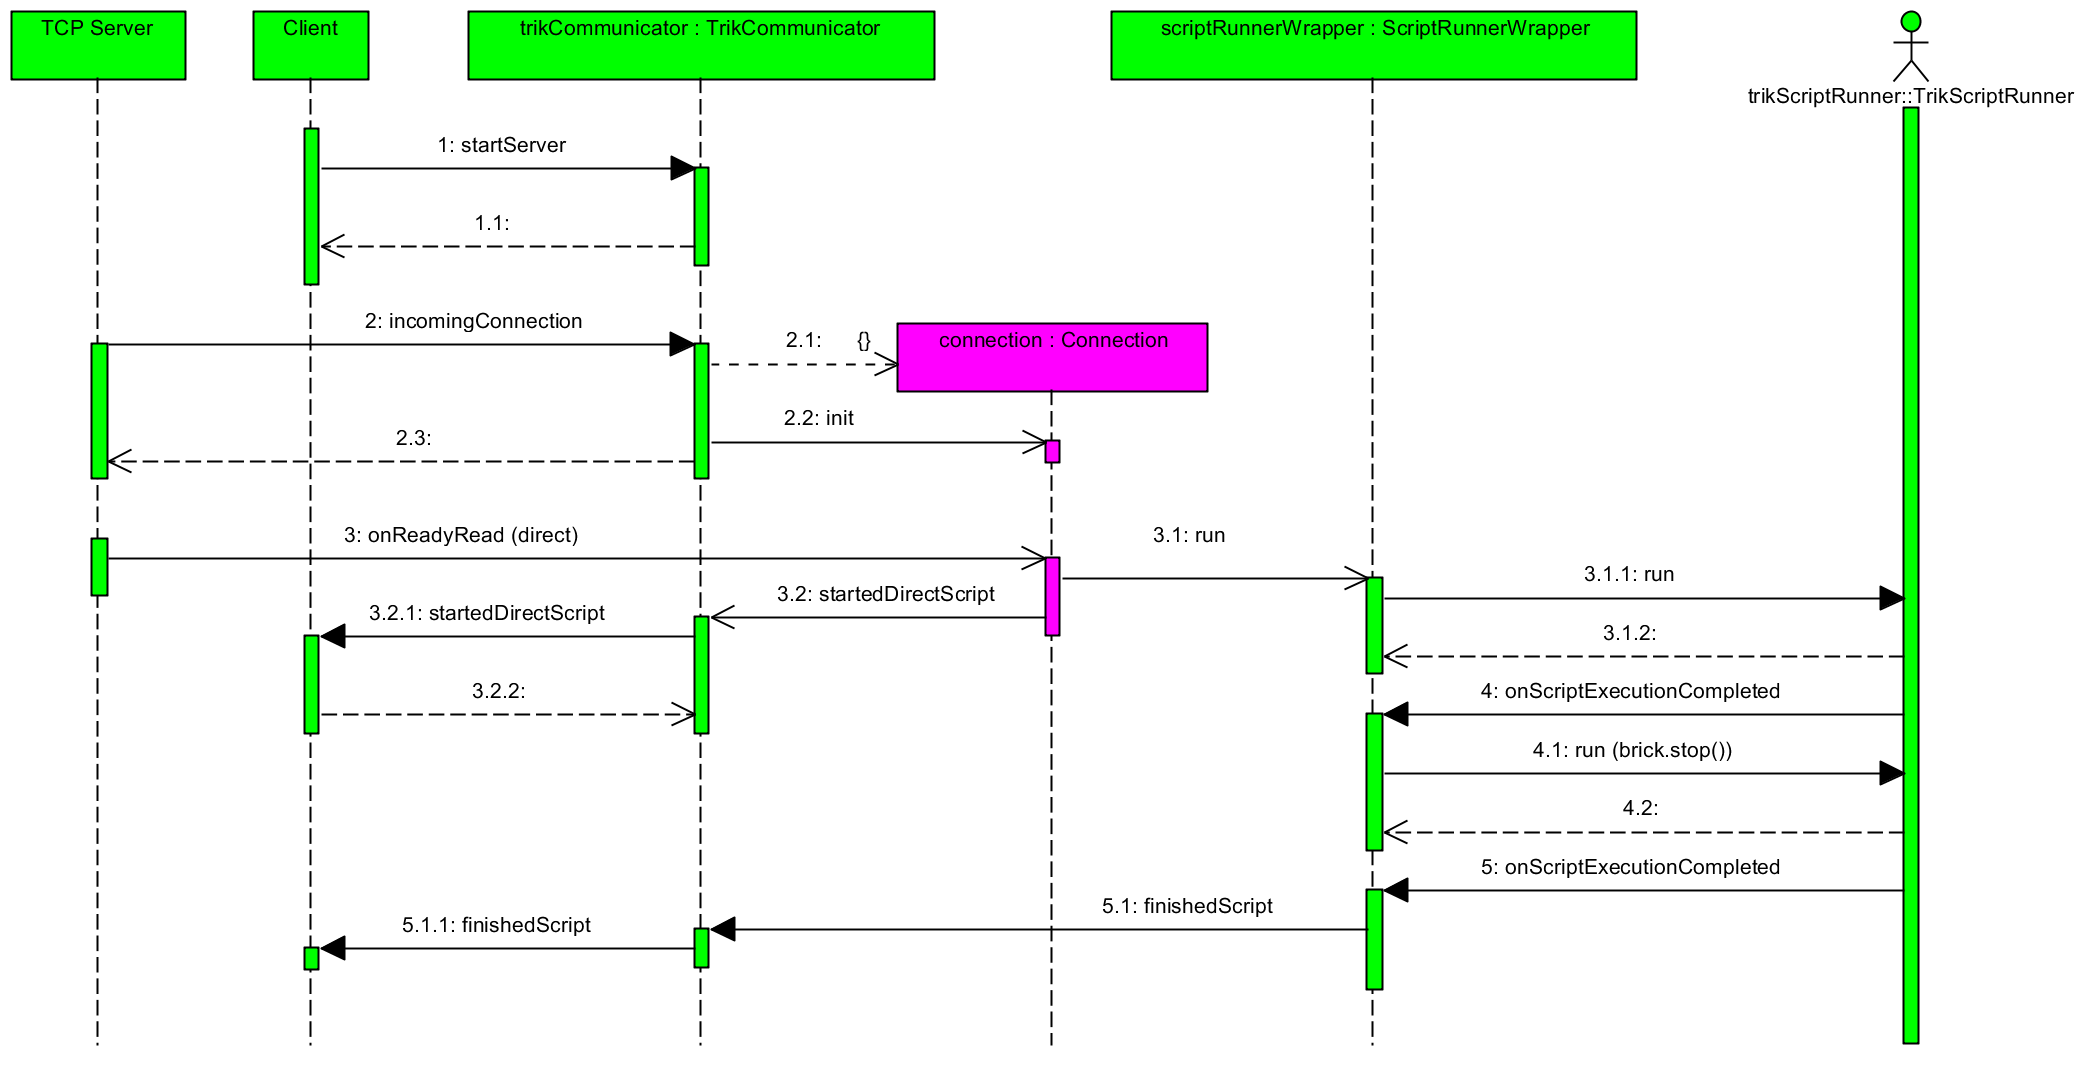
\includegraphics[width=0.8\textwidth]{sequenceDiagramExample2.png}
\end{center}

На сей раз это сценарий выполнения скрипта на роботе. Скрипт получается по сети, для чего сначала запускают сервер, ждут входящего соединения, создают в отдельном потоке объект для его обработки, и, как только скрипт полностью загружен, запускают его на исполнение. Когда скрипт заканчивает работу, мы получаем сигнал <<onScriptExecutionCompleted>>, после чего запускаем специальный скрипт остановки робота, который должен остановить все моторы и выключить все датчики. Уже после окончания этого скрипта мы посылаем клиенту сигнал о том, что всё закончилось.

В этом примере цветом выделен объект, живущий в отдельном потоке, стандарт UML этого не предписывает (но и не запрещает), на практике очень удобно.

И ещё один пример:

\begin{center}
	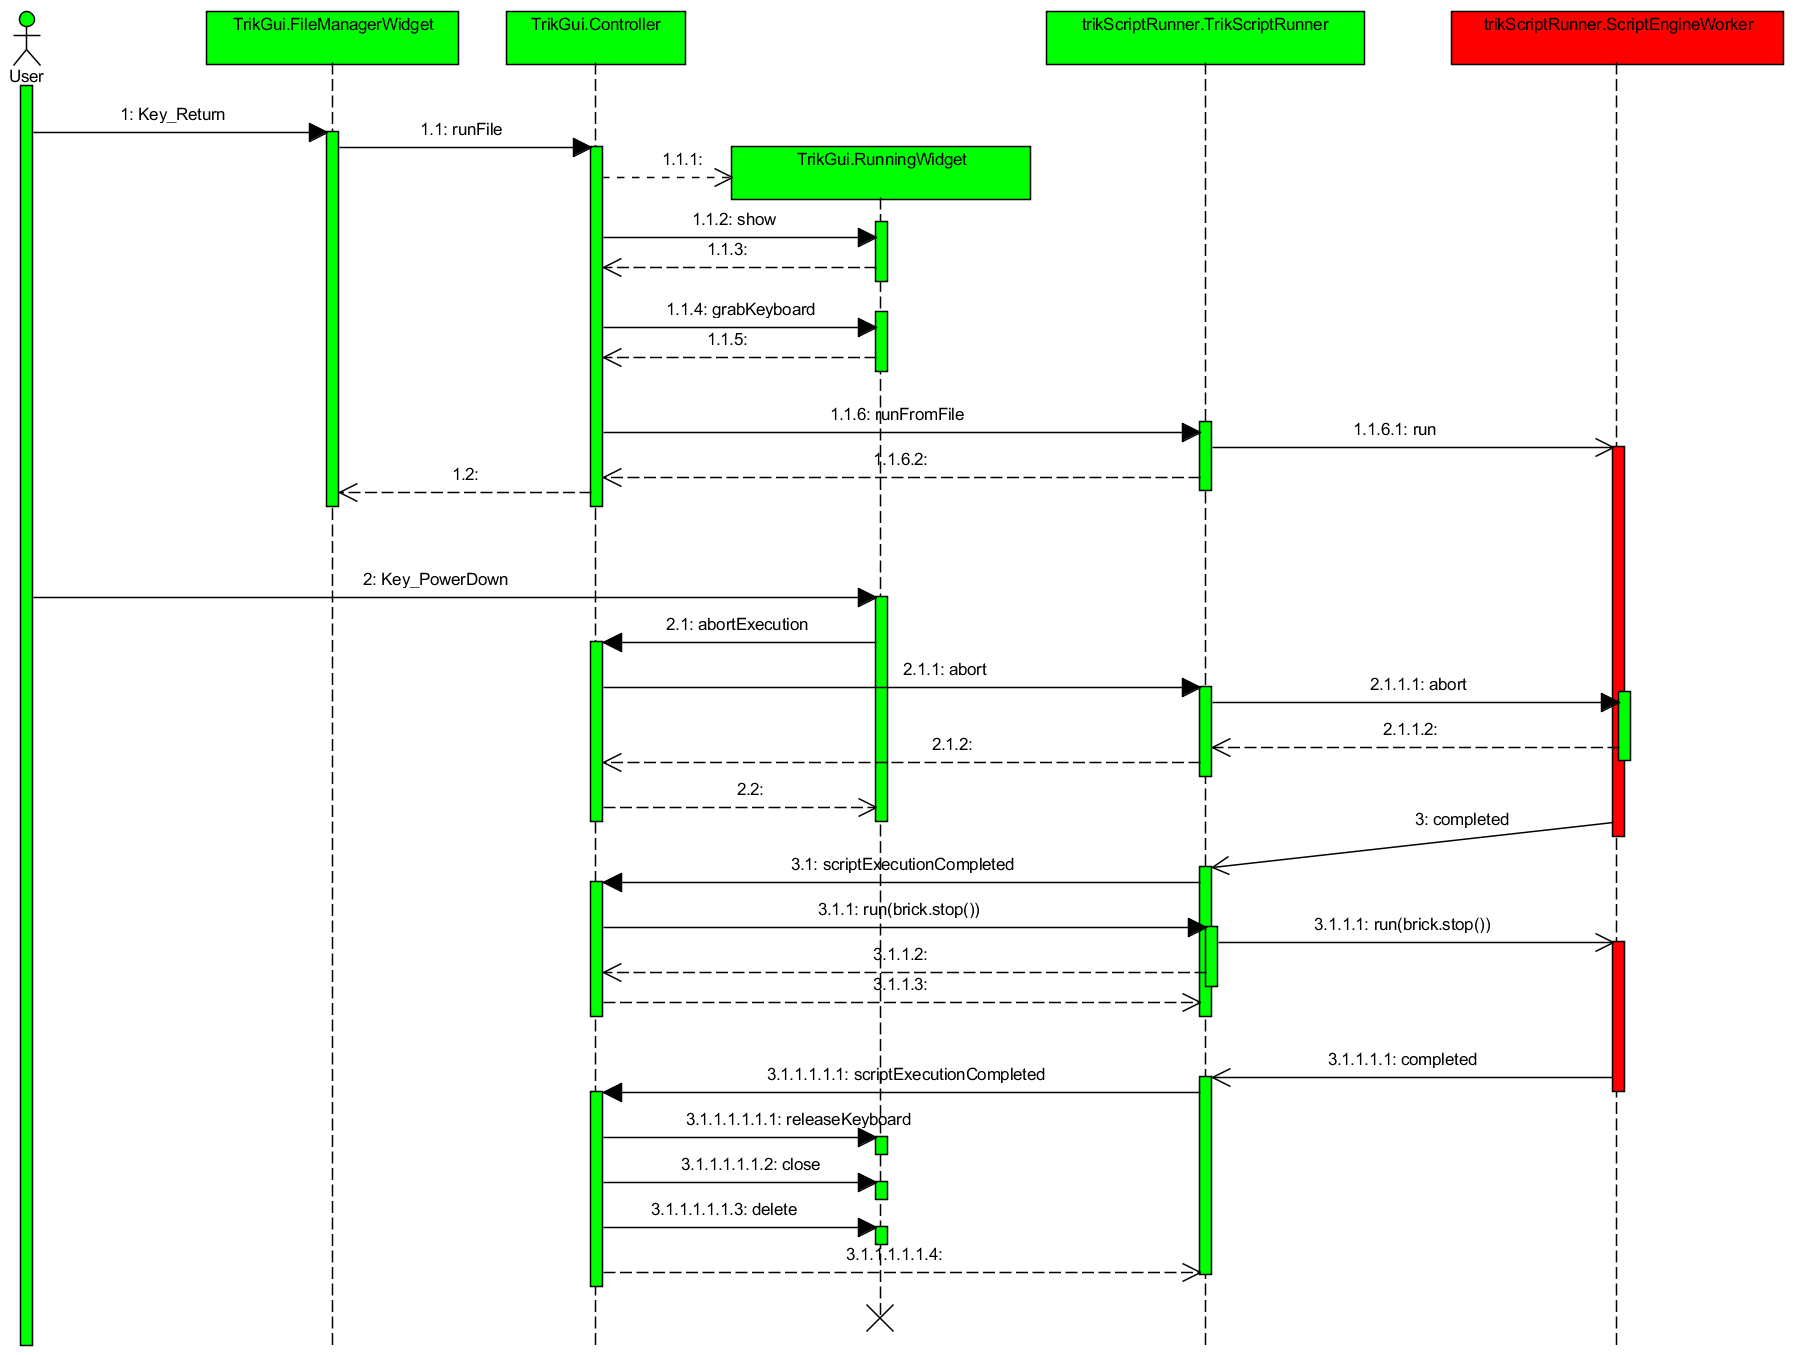
\includegraphics[width=0.8\textwidth]{sequenceDiagramExample3.png}
\end{center}

Это исполнение скрипта на роботе прямо с контроллера. Пользователь выбирает нужный скрипт в меню на экране робота, жмёт <<return>>, после этого инициализируется виджет, отображающий работу скрипта, скрипт запускается в отдельном потоке. Пользователь хочет прервать работу до её естественного окончания, он жмёт на <<powerDown>>, это посылает команду <<abort>> в поток со скриптом, он выполняет согласованную остановку и шлёт обратно <<completed>>. После этого запускается скрипт остановки робота, как в предыдущем примере. Как только он заканчивается, деинициализируем виджет исполнения скрипта и ждём следующие команды. Здесь тоже цветом выделен отдельный поток.

Все три примера взяты из проекта TrikStudio (\footnote{\url{https://github.com/trikset/trik-studio}}), где они показали себя как очень полезные для отладки и вообще понимания того, что происходит.

\subsection{Подробности синтаксиса}

На диаграмме также можно отобразить создание и удаление объекта:

\begin{center}
	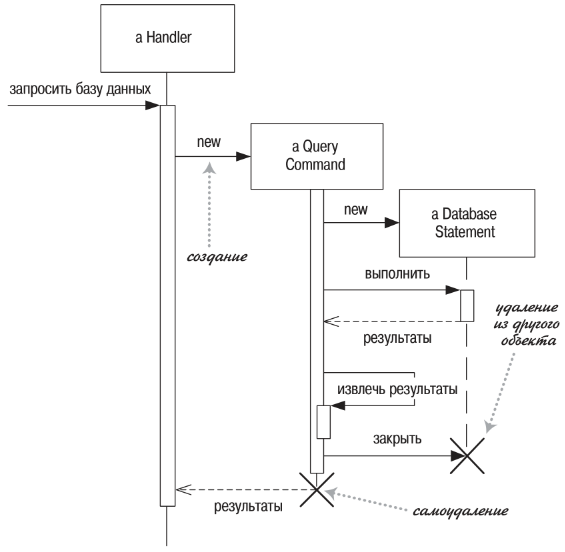
\includegraphics[width=0.5\textwidth]{sequenceDiagramCreationAndDeletion.png}
	\attribution{М. Фаулер, UML. Основы}
\end{center}

Создание означает, как правило, вызов конструктора, удаление более хитро --- либо это вызов деструктора, либо то место, где объект становится больше не нужен и его может собрать сборщик мусора. Создание инициирует другой объект, удаление --- либо сообщением от другого объекта, либо <<самоубийство>> в конце линии активации.

Все средства, описанные выше, позволяют задать только один конкретный сценарий взаимодействия, и обычно диаграммы последовательностей именно для этого и используются. Но если очень надо, можно попытаться отобразить целый алгоритм, с ветвлениями и циклами, с помощью фреймов. Например, псевдокод

\begin{minted}{text}
    foreach (lineitem)
        if (product.value > $10K)
            careful.dispatch
        else
            regular.dispatch
        end if
    end for
    if (needsConfirmation) 
        messenger.confirm
\end{minted}

на диаграмме может выглядеть как

\begin{center}
	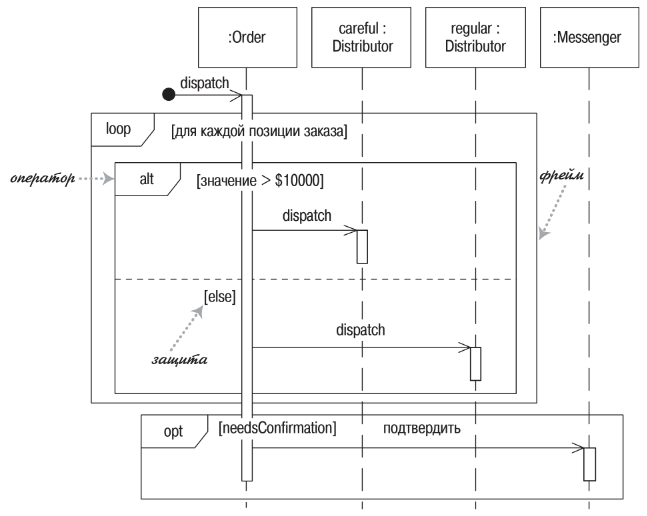
\includegraphics[width=0.5\textwidth]{sequenceDiagramFrames.png}
	\attribution{М. Фаулер, UML. Основы}
\end{center}

Фрейм ограничивает участок взаимодействия и позволяет исполнять его в цикле (фрейм <<loop>>), исполнять разные действия в зависимости от условия (фрейм <<alt>>, который играет роль if или switch/case, поскольку может иметь несколько разделов со взаимоисключающими условиями), просто исполнять или нет в зависимости от условия (фрейм <<opt>>).

Вообще фреймы сильно ухудшают читабельность диаграммы, а для визуализации алгоритмов есть средства получше --- диаграммы активностей, которые мы уже рассматривали, и диаграммы обзора взаимодействия, которые мы слегка рассмотрим дальше. Так что фреймы --- очень ситуационная штука.

\section{Коммуникационные диаграммы}

Коммуникационные диаграммы --- это по сути те же диаграммы последовательностей, только <<с высоты птичьего полёта>>. Они так же применяются для визуализации взаимодействия между объектами, так же подходят только для визуализации одного сценария взаимодействия и так же показывают последовательность обмена сообщениями:

\begin{center}
	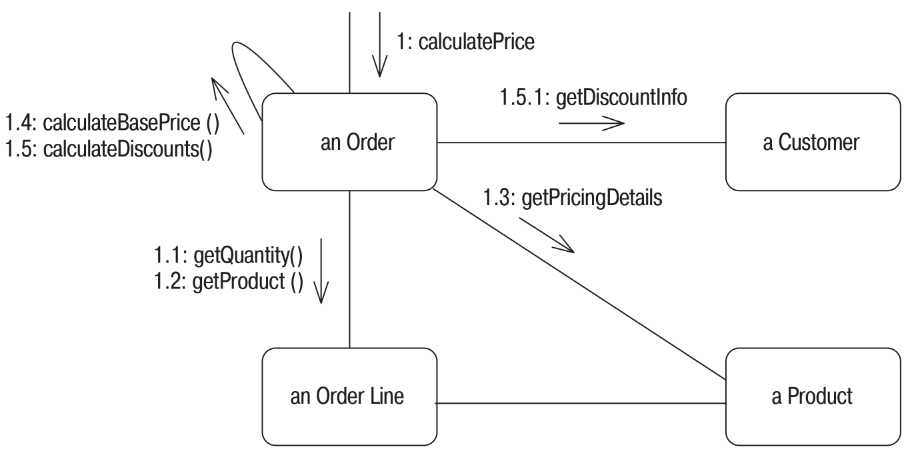
\includegraphics[width=0.6\textwidth]{communicationDiagram.png}
	\attribution{М. Фаулер, UML. Основы}
\end{center}

Однако если на ди

\end{document}
